
\section{Method}
\label{sec:method}
\begingroup
The construction has two stages (\docref{Figure}{fig:method}). During learning, the differential lifts of Neural Conservation Laws \citep{richterpowell2022neural} and potential boundary traces restrict the candidates to divergence-free, impermeable velocities. Geometry-local spectral orthogonalization follows Shape Space Spectra \citep{chang2025shapespacespectra}; harmonic circulation fields complete the span as in spectral fluid reduction \citep{liu2015model}. For a selected geometry, initial projection and preassembled Galerkin operators then turn this spatial basis into an autonomous coefficient model. The resulting state can be reconstructed at any requested spatial locations and output times.
\par\endgroup
\begin{figure}[!htb]
\centering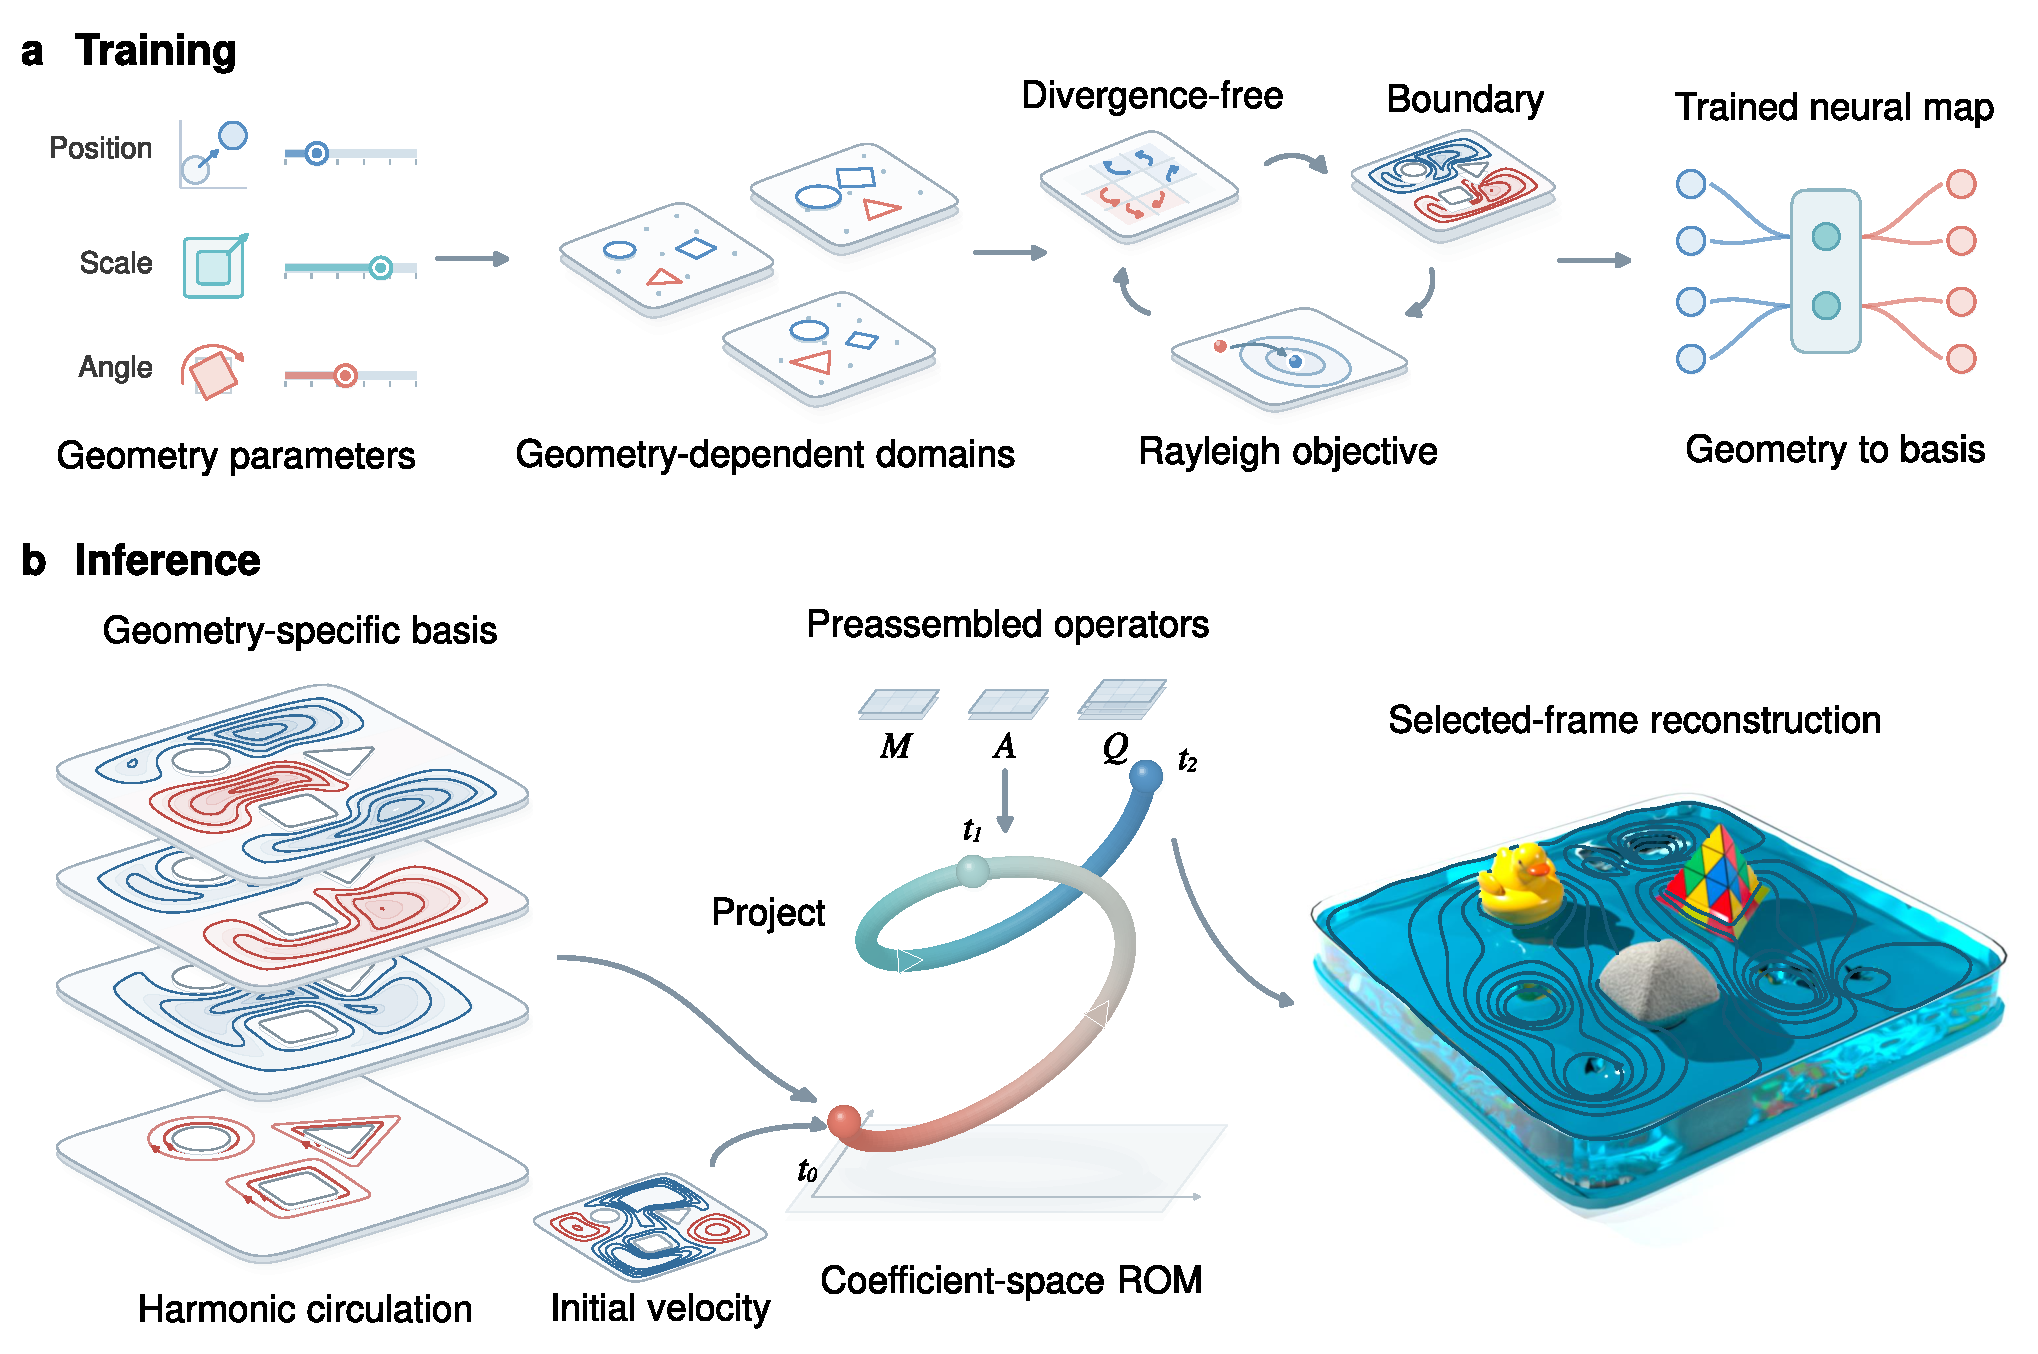
\includegraphics[width=\linewidth,height=.72\textheight,keepaspectratio]{unified_names_20261021_v1/method_overview.pdf}
\caption{\textbf{Shape-dependent training and coefficient-only inference.} (a) Geometry parameters vary obstacle position, scale and orientation within a fixed rounded-square outer boundary. A hard boundary envelope acts on geometry-conditioned potentials. Paired, oppositely oriented red and blue marks depict the antisymmetric tensor in the Neural Conservation Laws (NCL) construction {\citep{richterpowell2022neural}}; its row-wise divergence generates divergence-free velocities. {Gauge fixing and geometry-local causal orthogonalization produce normalized candidates within the divergence-free, impermeable trial space; the Rayleigh contours depict their energy minimization.} Training yields the parameter-to-basis neural map. (b) For a selected geometry, the map supplies positive modes, completed by harmonic circulation fields. Initial projection and geometry-specific preassembled mass, linear and quadratic operators support coefficient-only ROM stepping; spatial fields are reconstructed at selected times. The schematic uses $M$ for the velocity mass matrix, $A$ for the reduced linear operator, $Q$ for the quadratic advection tensor, and $t_0,t_1,t_2$ for selected output times. }
\label{fig:method}
\end{figure}


\subsection{The velocity space: positive modes and harmonic circulation}
Let $\Omega_{\mathbf g}\subset\R^D$ be a connected fluid domain of spatial dimension $D\in\{2,3\}$, indexed by geometry parameters $\mathbf g$, with outward unit normal $\mathbf n$. Here $\R$ is the real number space, $\mathbf x=(x_1,\ldots,x_D)$ is a spatial point, written $(x,y)$ in 2D or $(x,y,z)$ in 3D, and $\mathbf u$ denotes velocity. For scalar or vector fields $a,b$, we use the geometry-local mass inner product
\begin{equation}
\ip{a}{b}_{\mathbf g}=\int_{\Omega_{\mathbf g}}a\cdot b\,\dd\mathbf x,
\qquad \norm a_{\mathbf g}^2=\ip a a_{\mathbf g}.
\label{eq:metric}
\end{equation}
The dot is the Euclidean inner product (ordinary multiplication for scalars); $\dd\mathbf x$ is volume measure. For a fixed domain we write $\Omega=\Omega_{\mathbf g}$ and suppress the geometry subscript on the inner product and norm. The operators $\diver$ and $\curl$ denote spatial divergence and curl.
{An admissible velocity satisfies $\diver\mathbf u=0$ and $\mathbf u\cdot\mathbf n=0$: the wall is impermeable and tangential motion is permitted.} We order this space by vorticity energy in 2D and curl energy in 3D, giving the divergence-free absolute Hodge problem {\citep{arnold2006finite}}. Its zero-energy fields form the harmonic sector; its positive-energy eigenfields form the positive sector. To express both dimensions together, write $\alpha=\mathbf u^\flat$ for the velocity one-form, with $\flat$ the metric dual, $d$ for exterior differentiation, $\delta$ for its Hilbert adjoint, and $\star$ for the Hodge star. The contraction $\iota_{\mathbf n}$ extracts the normal trace. The subscript $A$ denotes absolute boundary conditions; the space $\Harm_A^1$ of harmonic velocity one-forms is
\begin{equation}
\Harm_A^1=\{\alpha:d\alpha=0,\ \delta\alpha=0,\ \iota_{\mathbf n}\alpha=0\}.
\label{eq:harmonic-space}
\end{equation}
These fields have zero Hodge energy but can carry circulation. For positive mode index $i$, let $\Phi_i$ be a normalized velocity eigenfield and $\lambda_i$ its eigenvalue. On admissible velocities orthogonal to the harmonic sector, they satisfy the weak eigenproblem for every admissible test field $v$:
\begin{equation}
\ip{d\Phi_i^\flat}{d v^\flat}=\lambda_i\ip{\Phi_i}{v},
\qquad \lambda_i>0,
\label{eq:target}
\end{equation}
\begingroup
The absolute Hodge realization has $\Phi_i\cdot\mathbf n=0$ and $\iota_{\mathbf n}d\Phi_i^\flat=0$; the latter is zero boundary vorticity in 2D and $\mathbf n\times\curl\Phi_i=0$ in 3D. These are the natural Hodge slip conditions of the spectral problem. The envelope imposes impermeability directly; the energy determines the natural eigenfield condition.
\par\endgroup

\subsection{Admissible neural potentials and the differential lift}
\begingroup
Geometry determines the domain, quadrature and boundary envelope. Following the geometry-conditioned spectral representation of \citet{chang2025shapespacespectra}, the network $f_\theta(\mathbf x,\mathbf g)$ has trainable parameters $\theta$ and outputs $K$ potential candidates $f_{\theta,i}$, indexed by $i=1,\ldots,K$, one per mode. The symbol $\widetilde\mu_i$ denotes the enveloped candidate before gauge selection and normalization: a scalar streamfunction in 2D and a vector potential in 3D. Geometry-family training samples $\mathbf g$ during optimization; fixed-domain training specializes this map to one geometry.
\par\endgroup

On a bounded domain we multiply each candidate by a differentiable geometry envelope $e_{\mathbf g}$ that vanishes on the domain boundary $\partial\Omega_{\mathbf g}$,
\begin{equation}
\widetilde\mu_i(\mathbf x,\mathbf g)=e_{\mathbf g}(\mathbf x)f_{\theta,i}(\mathbf x,\mathbf g),
\qquad e_{\mathbf g}|_{\partial\Omega_{\mathbf g}}=0.
\label{eq:envelope}
\end{equation}
The zero envelope enforces a sufficient relative potential trace: zero streamfunction trace in 2D and zero tangential vector-potential trace in 3D. The periodic benchmark uses a periodic encoding and identity envelope. For a potential $\mu$, write $\psi$ for its scalar streamfunction in 2D and $\mathbf A=(A_1,A_2,A_3)$ for its vector potential in 3D. With $\nabla$ the spatial gradient, $\partial_x,\partial_y$ coordinate derivatives, and $\nabla^\perp$ the rotated gradient, the potential-to-velocity map $\C=\star d$ specializes to
\begin{equation}
\mathbf u=\C\mu=
\begin{cases}
\nabla^\perp\psi=(\partial_y\psi,-\partial_x\psi),&D=2,\\
\curl\mathbf A,&D=3.
\end{cases}
\label{eq:lift}
\end{equation}
Equivalently, the Neural Conservation Laws (NCL) construction represents velocity as the row-wise divergence of an antisymmetric matrix field \citep{richterpowell2022neural}: $u_i=\sum_j\partial_j\mathsf S_{ij}$ with $\mathsf S=-\mathsf S^{\top}$. Here $u_i$ is velocity component $i$, $\partial_j$ differentiates coordinate $j$, the component indices run from $1$ to $D$, and $\top$ denotes transpose. For smooth fields, antisymmetry and commutation of mixed derivatives give
\begin{equation}
\diver\mathbf u=\frac12\sum_{i,j}\partial_i\partial_j
\bigl(\mathsf S_{ij}+\mathsf S_{ji}\bigr)=0.
\label{eq:ncl-antisymmetric}
\end{equation}
\begingroup
In 3D the equivalent antisymmetric potential is the $3\times3$ tensor $\mathsf S$. With $\epsilon_{ijk}$ the Levi--Civita symbol, normalized by $\epsilon_{123}=1$, its entries are $\mathsf S_{ij}=\sum_k\epsilon_{ijk}A_k$. In 2D, $\mathsf S_{12}=\psi$ and $\mathsf S_{21}=-\psi$.
\par\endgroup
These yield the rotated gradient and curl in \doceqref{eq:lift}, respectively. This cancellation is the coordinate form of $d^2=0$. In 2D a constant streamfunction trace has zero tangential derivative and hence zero normal velocity. In 3D the relative trace $\mathbf n\times\mathbf A=0$ gives a curl with zero normal component. Linear combinations preserve these identities, so the parameterization builds the kinematic constraints into the spectral trial space.

\begingroup
Several potentials generate the same velocity. Gauge fixing chooses one representative so that its mass norm, orthogonalization and Rayleigh objective measure the flow-producing coordinates consistently.
\par\endgroup

\subsection{Gauge representatives and the potential metric}
\label{sec:gauge}
\paragraph{Scalar constants in 2D.}
{Periodic streamfunctions admit the constant freedom $\nabla^\perp(\psi+c)=\nabla^\perp\psi$. Here $c$ is an arbitrary scalar constant. We select the centered representative $\psi^\circ$ by subtracting the area-weighted mean $\langle\psi\rangle_\Omega$. Its quadrature approximation uses the node--weight set $Q=\{(\mathbf x_q,w_q)\}_q$, with node index $q$ and positive weights $w_q$:}
\begin{equation}
\psi^\circ=\psi-\langle\psi\rangle_\Omega,
\qquad \langle\psi\rangle_{\Omega,Q}=\frac{\sum_q w_q\psi(\mathbf x_q)}{\sum_q w_q}.
\label{eq:scalar-gauge}
\end{equation}
{This centering removes the constant null coordinate before normalization, ordering, and Gram--Schmidt, and is differentiated during training. It makes the potential norm measure the spatially varying field: an unconstrained constant could otherwise lower the Rayleigh ratio arbitrarily without changing velocity.}


For the bounded scalar Dirichlet problem, $\psi=0$ on the boundary selects the representative. The multi-hole experiment uses this boundary-pinned mass norm. Scalar-field displays subtract one global spatial mean, preserving derivatives and circulation while giving the plots a common gauge. \docref{Appendix}{app:scalar} details the distinction between the boundary-pinned training metric and the centered display convention.

\paragraph{Curl-free directions in 3D.}
{The vector-potential gauge kernel contains admissible gradients and may also contain relative harmonic fields. We first remove the gradients with a Coulomb projection, as also used in vector-potential fluid editing \citep{chen2026obstacle}. Let $\widetilde{\mathbf A}$ be the raw potential, $\phi$ its scalar gauge correction, $\Delta=\nabla\cdot\nabla$ the Laplacian, and $\mathbf A'$ the gradient-corrected field:}
\begin{equation}
\Delta\phi=\diver\widetilde{\mathbf A},\qquad \phi|_{\partial\Omega}=0,
\qquad \mathbf A'=\widetilde{\mathbf A}-\nabla\phi,
\label{eq:poisson-gauge}
\end{equation}
We then obtain the canonical potential $\mathbf A^\circ$ using the identity operator $I$ and the mass-orthogonal projector $P_{\Harm_R^1}$ onto the relative harmonic potential space $\Harm_R^1$ (the subscript $R$ denotes relative boundary conditions):
\begin{equation}
\mathbf A^\circ=(I-P_{\Harm_R^1})\mathbf A'.
\label{eq:vector-gauge}
\end{equation}
The exact representative is orthogonal to the kernel of $\C$, has zero divergence, and preserves curl and the relative boundary trace. A geometry-dependent solve handles all mode right-hand sides together. For the Metaball Potential objective (the canonical curl quotient), the full relative compatible curl complex selects the mass-orthogonal canonical representative, with physical solve actions in FP64. The Gauge-Constrained Potential (GCP) controls use distinct gauge treatments: augmented-Lagrangian constraints (Potential-AL) and finite scalar/harmonic projection (Potential-FG), as detailed in \docref{Appendix}{app:old-Pot}. The removed relative harmonic \emph{potential} fields $\Harm_R^1$ belong to the gauge kernel. The absolute harmonic \emph{velocity} fields $\Harm_A^1$ carry physical circulation and enter the completed velocity basis.


\subsection{Rayleigh learning and the effect of objective choice}
Denote the selected potential representative by $\mu^\dagger$: canonical for the periodic/vector quotient and boundary-pinned for the scalar Dirichlet experiment. {Following variational neural eigenfunction learning \citep{e2018deep,pfau2019spectral,rowan2025rayleigh}, the potential Rayleigh ratio $R_p$ and its Hodge velocity counterpart $R_v$ are}
\begin{equation}
R_p(\mu^\dagger)=\frac{\norm{\C\mu^\dagger}^2}{\norm{\mu^\dagger}^2},
\qquad R_v(\mu^\dagger)=\frac{\norm{d(\C\mu^\dagger)}^2}{\norm{\C\mu^\dagger}^2}.
\label{eq:rayleigh}
\end{equation}
For a streamfunction these are $\norm{\nabla\psi^\dagger}^2/\norm{\psi^\dagger}^2$ and $\norm{\Delta\psi}^2/\norm{\nabla\psi}^2$. For a canonical vector potential they are $\norm{\curl\mathbf A^\circ}^2/\norm{\mathbf A^\circ}^2$ and $\norm{\curl\curl\mathbf A^\circ}^2/\norm{\curl\mathbf A^\circ}^2$. We use \textbf{Potential} for potential-space Rayleigh training and \textbf{Velocity} for velocity-space Rayleigh training. Potential uses a scalar streamfunction in 2D and the mass-orthogonal canonical vector potential in 3D. Velocity optimizes the energy and mass of the lifted velocity; its network can still parameterize a potential before the differential lift. \textbf{Laplacian} denotes the numerically solved spectral basis, and \textbf{NKB} denotes the direct-velocity Neural Kinematic Basis. The potential controls are named \textbf{Potential-FG} for finite scalar/harmonic gauge projection and \textbf{Potential-AL} for augmented-Lagrangian constraints. The potential form therefore uses one fewer spatial derivative. Both variational energies learn the operator-defined coordinates directly from geometry and spatial derivatives.

The lower-order objective is linked to the velocity spectrum by the differential lift. Write $\C^*$ for the mass-inner-product adjoint of $\C$, and $\mu_i$ for a normalized potential eigenmode. If $\C^*\C\mu_i=\lambda_i\mu_i$ with $\lambda_i>0$ and $\norm\mu_i=1$, then
\begin{equation}
\Phi_i=\frac{\C\mu_i}{\sqrt{\lambda_i}},\qquad
\C\C^*\Phi_i=\lambda_i\Phi_i,\qquad \norm{\Phi_i}=1.
\label{eq:paired-lift}
\end{equation}
\begingroup
Under compatible relative/absolute domains, $\C\C^*$ is the positive Hodge velocity operator. The classical Hodge pairing gives the same exact nonzero spectrum, including multiplicities \citep{arnold2006finite}. This includes mean-zero periodic fields and decaying free-space fields when integration by parts has no boundary contribution. The equivalence concerns eigenvalues and their lifted eigenspaces; for arbitrary approximate candidates the objectives obey \doceqref{eq:variance}. \docref{Appendix}{app:spectrum} gives the operator proof and its free-space specialization.
\par\endgroup


The objectives still differ away from an exact eigenspace. For a potential expansion $\mu=\sum_j a_j\mu_j$, with spectral coefficients $a_j$ and mode index $j$ in an orthonormal potential eigenbasis,
\begin{equation}
R_p=\frac{\sum_j\lambda_j|a_j|^2}{\sum_j|a_j|^2},\qquad
R_v=\frac{\sum_j\lambda_j^2|a_j|^2}{\sum_j\lambda_j|a_j|^2}\ge R_p.
\label{eq:moments}
\end{equation}
Writing $p_j=|a_j|^2/\sum_\ell|a_\ell|^2$ defines probability weights on the eigenvalues. With $\mathbb E_p$ and $\operatorname{Var}_p$ denoting their weighted mean and variance, the difference is
\begin{equation}
R_v-R_p=\frac{\operatorname{Var}_p(\lambda)}{\mathbb E_p[\lambda]}.
\label{eq:variance}
\end{equation}
Velocity learning places extra weight on high-frequency content in an approximate mode. This changes the optimization of a finite neural representation even though the exact spectra agree. The periodic experiment measures the resulting cost--accuracy tradeoff. \docref{Appendix}{app:spectrum} derives the correspondence and the boundary term relating componentwise gradient energy to curl energy in 3D.

\subsection{Geometry-local ordering and causal orthogonalization}
Multiple independent outputs must span distinct low-frequency directions. For quadrature points $(\mathbf x_q,w_q)$ with $w_q>0$, define
\begin{equation}
\ip{a}{b}_Q=\sum_q w_q a(\mathbf x_q)\cdot b(\mathbf x_q).
\end{equation}
At each sampled geometry we select representatives, normalize them in the chosen metric, and sort detached preliminary Rayleigh values. The geometry-local permutation $\pi$ adapts the ordering to that domain. Let $\bar\mu_i$ be preliminary normalized representatives, $\nu_i$ their orthogonalization residuals, and $\widehat\mu_i$ the resulting unit-norm candidates, where $\|a\|_Q^2=\langle a,a\rangle_Q$. The operator $\sg$ stops differentiation through its argument. The training loss $\mathcal L(\theta)$ averages the quadrature Rayleigh ratio $R_{p,Q}$ over the sampled geometry distribution, denoted by $\mathbb E_{\mathbf g}$. For the potential objective, causal orthogonalization follows Shape Space Spectra \citep{chang2025shapespacespectra} and treats lower-ranked modes as fixed when learning the next mode:
\begin{align}
\nu_i&=\bar\mu_{\pi(i)}-\sum_{j<i}\ip{\bar\mu_{\pi(i)}}{\sg(\widehat\mu_j)}_Q\sg(\widehat\mu_j),\\
\widehat\mu_i&=\nu_i/\norm{\nu_i}_Q,
\qquad \mathcal L(\theta)=\mathbb E_{\mathbf g}\sum_{i=1}^K R_{p,Q}(\widehat\mu_i).
\label{eq:training}
\end{align}
A second orthogonalization pass reduces accumulated projection error. The causal gradient prevents a higher mode from changing a lower mode merely to simplify its own residual. Because gauge selection and the boundary constraints define linear spaces, the subsequent linear combinations preserve them.

The velocity objective uses the velocity inner product and corresponding energy, applying the same coefficient transform to every derivative channel. Spatial derivatives and parameter adjoints use an analytic CuPy implementation. At repeated eigenvalues, the identifiable object is the eigenspace; the mode atlas is interpreted up to signs and orthogonal rotations within that space.

\begin{figure}[!t]
\centering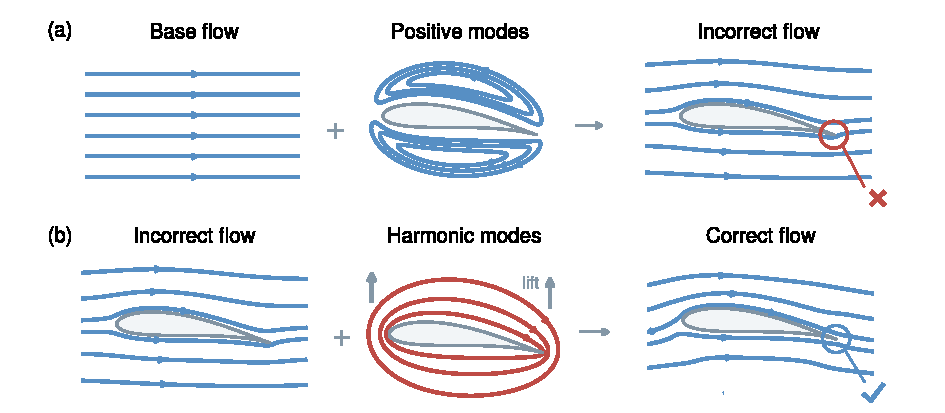
\includegraphics[width=0.7\linewidth,height=.72\textheight,keepaspectratio]{unified_names_20261021_v1/harmonic_airfoil.pdf}
\caption{\textbf{Harmonic circulation completes the flow representation.} (a) A base flow combined with positive modes gives an incomplete, zero-circulation description of a lifting airfoil, with an incorrect sharp-trailing-edge flow. (b) Adding harmonic circulation permits smooth outflow satisfying the Kutta condition and generates lift in the presence of the base flow. Streamlines schematically illustrate the decomposition in \doceqref{eq:completion}.}
\label{fig:harmonic-airfoil}
\end{figure}

\subsection{Harmonic completion at fixed capacity}
\label{sec:rom}
{Harmonic zero-frequency fields complete the spectral ROM basis in \citet{liu2015model}. We construct their neural counterparts with a dedicated boundary-value objective. Zero-trace positive streamfunctions describe the vortical sector; independent curl-free circulation is supplied by differences between boundary constants. Let $h$ be the number of holes, $\Gamma_0$ the outer boundary, and $\Gamma_m$ the boundary of obstacle $m=1,\ldots,h$. For obstacle $\ell$, its harmonic measure $\chi_\ell$ solves the following problem, where $\delta_{\ell m}$ is the Kronecker delta:}
\begin{equation}
\Delta\chi_\ell=0,\qquad
\chi_\ell|_{\Gamma_m}=\delta_{\ell m},\qquad
\chi_\ell|_{\Gamma_0}=0,
\label{eq:harmonic-measure}
\end{equation}
The velocities $h_\ell=\nabla^\perp\chi_\ell$ are divergence-free, curl-free, and tangent to every boundary. Their span has one independent coordinate per hole. Cardinal boundary values are convenient coordinates; a further invertible circulation matrix can convert them into unit-period coordinates.

{Let $L_\ell$ be a fixed lift of the cardinal boundary traces and $n_{\theta,\ell}$ a neural correction. The parameterization $\chi_\ell=L_\ell+e_{\mathbf g}n_{\theta,\ell}$ gives the correction zero trace. The harmonic training loss $\mathcal L_H$ therefore minimizes Dirichlet energy within this prescribed boundary-value space:}
\begin{equation}
\mathcal L_H(\theta;\mathbf g)=\sum_{\ell=1}^{h}\int_{\Omega_{\mathbf g}}|\nabla\chi_\ell|^2\,\dd\mathbf x,
\label{eq:harmonic-loss}
\end{equation}
{Fixed traces determine the scale of a harmonic measure, so this numerator-only objective directly realizes the Dirichlet principle through neural energy minimization \citep{e2018deep}. \docref{Appendix}{app:harmonic-loss} gives the variational derivation. Raw and scaled lifts parameterize the same boundary-value problem and correction space with different optimization coordinates. Holding the positive checkpoint fixed while changing the lift isolates this conditioning effect.}

With $h$ holes and total dimension $K$, the completed representation contains $K-h$ positive modes and $h$ harmonic modes. Let $\mathbf u_{\rm base}$ supply any prescribed base flow, and $a_i,b_\ell$ be the positive and harmonic coefficients:
\begin{equation}
\mathbf u=\mathbf u_{\rm base}+\sum_{i=1}^{K-h}a_i\Phi_i+\sum_{\ell=1}^{h}b_\ell h_\ell.
\label{eq:completion}
\end{equation}
The prescribed base flow carries nonhomogeneous data when present. Writing $P_K=\operatorname{span}\{\Phi_1,\ldots,\Phi_K\}$ and $H_h=\operatorname{span}\{h_1,\ldots,h_h\}$, the comparison $P_K$ versus $P_{K-h}+H_h$ changes the allocation of coordinates while keeping their total number fixed. We abbreviate these allocations as P and P+H (or PH). They test topological completeness at the same capacity. \docref{Appendix}{app:topology-rom} illustrates this distinction on an annulus and gives the circulation normalization.

\begingroup
Circulation is particularly important in lifting-airfoil flow. In the ideal slip-flow illustration of \docref{Figure}{fig:harmonic-airfoil}, the Kutta condition selects a circulation $\Gamma$ and the classical Kutta--Joukowski lift per unit span has magnitude $\rho U_\infty|\Gamma|$, where $\rho$ is fluid density and $U_\infty$ the freestream speed \citep{batchelor2000fluid}. The harmonic coordinate permits that circulation to be represented alongside the base flow and positive modes. This motivates including the sector whenever the target physics requires it; the multi-hole experiments quantify its allocation at a fixed coordinate budget.
\par\endgroup

\subsection{From the learned span to autonomous dynamics}
{Write the reduced velocity as $u=u_{\rm base}+Uc$, where column $U_i$ is basis field $i$ and $c=(c_1,\ldots,c_K)^{\top}$ is the coefficient state. Following spectral fluid Galerkin reduction \citep{dewitt2012fluid,liu2015model}, let $t$ denote simulation time and $\dot c=\dd c/\dd t$. The full velocity mass matrix $M$ defines the coefficient metric, the vorticity/curl stiffness matrix $S$ supplies viscous dissipation, $\nu$ is kinematic viscosity, and $Q(c,c)$ is the quadratic advective load. Projection of the homogeneous unforced Hodge model gives}
\begin{equation}
M\dot c=Q(c,c)-\nu S c,\qquad
M_{ij}=\ip{U_i}{U_j},\quad S_{ij}=\ip{dU_i^\flat}{dU_j^\flat},
\label{eq:reduced-dynamics}
\end{equation}
\begingroup
For indices $i,j,k=1,\ldots,K$, advection gives the quadratic load $[Q(c,c)]_i=\sum_{j,k}Q_{ijk}c_jc_k$, with $Q_{ijk}=-\langle U_i,(U_j\cdot\nabla)U_k\rangle$.
\par\endgroup
{A base flow or force contributes the corresponding constant and linear terms. Exact orthonormal eigenfields make $M$ the identity and $S$ diagonal. For the learned span, retaining the full operators incorporates its measured metric and energy couplings into the dynamics.}

For initial velocity $u_0$, the initial coefficients solve $M c(0)=\ip{U}{u_0-u_{\rm base}(0)}$, where the vector inner product has entry $\langle U_i,u_0-u_{\rm base}(0)\rangle$. This initializes an autonomous coefficient trajectory. Numerical reference states enter the subsequent error measurement. Learned and numerical bases use the same stated discrete generator within each matched comparison, including the normal-penalty grid generator in 3D.

\paragraph{Offline assembly and coefficient-only integration.}
For a fixed span and a quadratic discrete fluid generator, {preassembled reduced operators \citep{treuille2006model,dewitt2012fluid,liu2015model} move full-field evaluation offline. Here $\mathcal L$ denotes the specified linear fluid generator (viscosity and any linear penalty or base-flow terms), while $\mathcal N$ denotes its bilinear advective part. Writing the generator as $\mathcal L u+\mathcal N(u,u)$ gives the reduced linear matrix $A$ and quadratic tensor $\mathcal Q$ below. The subscript $h$ denotes the discrete spatial quadrature:}
\begin{equation}
M\dot c=A c+\mathcal Q(c,c),\qquad
A_{ij}=\ip{U_i}{\mathcal L U_j}_h,\quad
\mathcal Q_{ijk}=\ip{U_i}{\mathcal N(U_j,U_k)}_h.
\label{eq:offline-rom}
\end{equation}

The same quadrature defines $M$ and the two assembled operators. During inference, each time-integration stage contracts these fixed operators with the current coefficient vector and solves the full mass system using its cached Cholesky factor. The recurrent state is therefore the reduced vector $c(t)$ throughout the trajectory. Spatial reconstruction $u(t)=u_{\rm base}(t)+Uc(t)$ is performed only at requested output times, as illustrated in \docref{Figure}{fig:method}. This is an algebraic reorganization of the chosen Galerkin system. \docref{Appendix}{app:coefficient-acceleration} measures operator equivalence, integration time, offline cost, and flow error separately.

